\documentclass[border=8pt,varwidth=16cm]{standalone}
\usepackage[utf8]{inputenc}
\usepackage[T1]{fontenc}
\usepackage[turkish,shorthands=:!]{babel}
\usepackage{lmodern}
\usepackage{amsmath}
\usepackage{tikz}
\usetikzlibrary{arrows.meta,positioning,babel}
\usepackage[american]{circuitikz}
\begin{document}
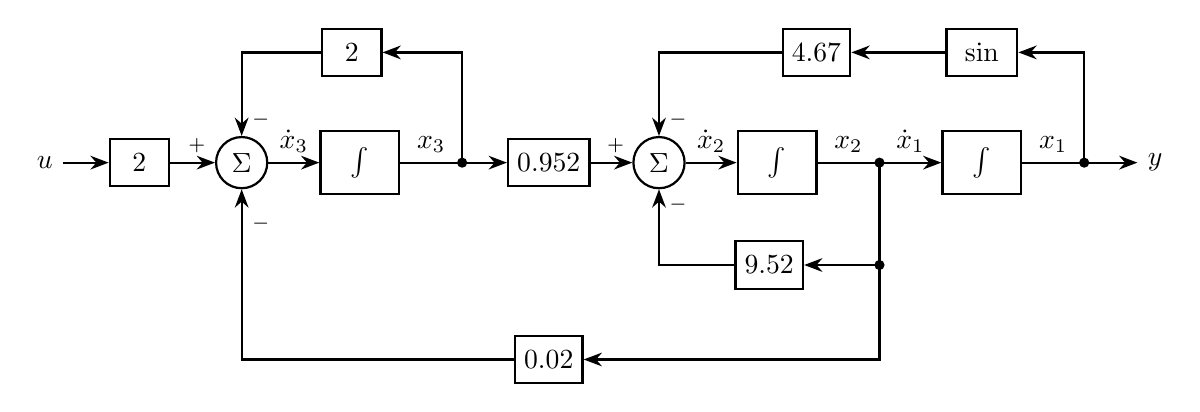
\begin{tikzpicture}[>=Stealth, thick,
  integ/.style={draw, minimum width=1.0cm, minimum height=0.8cm},
  sumb/.style={draw, circle, inner sep=0pt, minimum size=0.65cm},
  gain/.style={draw, minimum width=0.75cm, minimum height=0.6cm},
  dot/.style={circle, fill, inner sep=1.3pt},
  sgn/.style={font=\scriptsize}]
  % ileri yol
  \node (u) at (0,0) {$u$};
  \node[gain]  (gu)  at (1.2,0)  {$2$};
  \node[sumb]  (s3)  at (2.5,0)  {$\Sigma$};
  \node[integ] (i3)  at (4.0,0)  {$\int$};
  \coordinate  (c3)  at (5.3,0);
  \node[gain]  (gk)  at (6.4,0)  {$0.952$};
  \node[sumb]  (s2)  at (7.8,0)  {$\Sigma$};
  \node[integ] (i2)  at (9.3,0)  {$\int$};
  \coordinate  (c2)  at (10.6,0);
  \node[integ] (i1)  at (11.9,0) {$\int$};
  \coordinate  (c1)  at (13.2,0);
  \node (y) at (14.1,0) {$y$};
  \draw[->] (u) -- (gu);
  \draw[->] (gu) -- node[sgn, above, pos=0.6]{$+$} (s3);
  \draw[->] (s3) -- node[above]{$\dot x_3$} (i3);
  \draw (i3) -- node[above]{$x_3$} (c3);
  \draw[->] (c3) -- (gk);
  \draw[->] (gk) -- node[sgn, above, pos=0.6]{$+$} (s2);
  \draw[->] (s2) -- node[above]{$\dot x_2$} (i2);
  \draw (i2) -- node[above]{$x_2$} (c2);
  \draw[->] (c2) -- node[above]{$\dot x_1$} (i1);
  \draw (i1) -- node[above]{$x_1$} (c1);
  \draw[->] (c1) -- (y);
  \node[dot] at (c3) {}; \node[dot] at (c2) {}; \node[dot] at (c1) {};
  % x3 -> sargi direnci (ust)
  \node[gain] (gr) at (3.9,1.4) {$2$};
  \draw[->] (c3) |- (gr);
  \draw[->] (gr) -| node[sgn, pos=0.9, right]{$-$} (s3);
  % x1 -> sin -> yercekimi (ust)
  \node[draw, minimum width=0.9cm, minimum height=0.6cm] (sn) at (11.9,1.4) {$\sin$};
  \node[gain] (gg) at (9.8,1.4) {$4.67$};
  \draw[->] (c1) |- (sn);
  \draw[->] (sn) -- (gg);
  \draw[->] (gg) -| node[sgn, pos=0.9, right]{$-$} (s2);
  % x2 -> surtunme (alt)
  \coordinate (d2) at (10.6,-1.3);
  \node[gain] (gb) at (9.2,-1.3) {$9.52$};
  \draw (c2) -- (d2);
  \node[dot] at (d2) {};
  \draw[->] (d2) -- (gb);
  \draw[->] (gb) -| node[sgn, pos=0.9, right]{$-$} (s2);
  % x2 -> zit EMK (en alt)
  \node[gain] (ge) at (6.4,-2.5) {$0.02$};
  \draw[->] (d2) |- (ge);
  \draw[->] (ge) -| node[sgn, pos=0.9, right]{$-$} (s3);
\end{tikzpicture}
\end{document}
